% Harus dimuat terlebih dahulu, digunakan agar file PDF memiliki format karakter yang benar.
% Untuk informasi lebih lanjut, lihat https://ctan.org/pkg/cmap.
\RequirePackage{cmap}

% Format dokumen sebagai paper konferensi menggunakan aturan IEEEtran terbaru (v1.8b).
% Untuk informasi lebih lanjut, lihat http://www.michaelshell.org/tex/ieeetran/.
\documentclass[conference]{IEEEtran}[2015/08/26]

% Format encoding font dan input menjadi 8-bit UTF-8.
\usepackage[T1]{fontenc}
\usepackage[utf8]{inputenc}

% Format bahasa menjadi bahasa german dan inggris.
\usepackage[english]{babel}

% Digunakan untuk tujuan demonstrasi.
\usepackage{mwe}

% Digunakan untuk menampilkan font dengan style yang lebih baik.
\usepackage[zerostyle=b,scaled=.75]{newtxtt}

% Digunakan untuk menampilkan tabel dengan style yang lebih baik.
\usepackage{booktabs}

% Digunakan untuk menampilkan gambar pada dokumen.
\usepackage{graphicx}

% Digunakan untuk menampilkan potongan kode.
\usepackage{listings}
\lstset{
  basicstyle=\ttfamily,
  columns=fixed,
  basewidth=.5em,
  xleftmargin=0.5cm,
  captionpos=b
}

% Digunakan agar backticks (`) dapat dirender pada PDF.
% Untuk informasi lebih lanjut, lihat https://tex.stackexchange.com/a/341057/9075.
\usepackage{upquote}

% Digunakan untuk menyeimbangkan bagian akhir dokumen dengan dua kolom.
\usepackage{balance}

\usepackage{multirow}
\usepackage{adjustbox}
\usepackage{graphicx}
\usepackage{placeins}

% Digunakan untuk menampilkan pustaka.
\usepackage[square,comma,numbers,sort&compress]{natbib}

% Mengubah format ukuran teks pada natbib.
\renewcommand{\bibfont}{\normalfont\footnotesize}

% Menambah nama penulis ketika menggunakan perintah \citet.
% Untuk informasi lebih lanjut, lihat https://tex.stackexchange.com/a/76075/9075.
\usepackage{etoolbox}
\makeatletter
\patchcmd{\NAT@test}{\else \NAT@nm}{\else \NAT@hyper@{\NAT@nm}}{}{}
\makeatother

% Digunakan untuk melakukan linewrap pada pustaka dengan url yang panjang
% jika terdapat hyphens
\usepackage[hyphens]{url}

% Digunakan untuk menambah hyperlink pada referensi.
\usepackage{hyperref}

% Menonaktifkan warna dan bookmark pada hyperref.
\hypersetup{hidelinks,
  colorlinks=true,
  allcolors=black,
  pdfstartview=Fit,
  breaklinks=true
}

% Digunakan untuk membenarkan hyperref pada gambar.
\usepackage[all]{hypcap}

% Digunakan untuk menampilkan beberapa gambar
\usepackage[caption=false,font=footnotesize]{subfig}

\usepackage{stfloats}

% Tambahkan format tanda hubung yang benar di sini
\hyphenation{
  ro-ket
  me-ngem-bang-kan
  per-hi-tu-ngan
}

\begin{document}

  % Ubah kalimat berikut sesuai dengan judul penelitian.
\title{Deteksi Helm Keselamatan Kerja Menggunakan CNN}

% Ubah kalimat-kalimat berikut sesuai dengan nama, institusi, alamat dan kontak penulis.
\author{
  \IEEEauthorblockN{Helmika Mahendra P.}
  \IEEEauthorblockA{Departemen Teknik Komputer\\
    Fakultas Teknologi Elektro dan Informatika Cerdas\\
    Institut Teknologi Sepuluh Nopember\\
    Surabaya, Indonesia 60111\\
    helmikapriyanto.18072@mhs.its.ac.id}

  \and
  \IEEEauthorblockN{Reza Fuad Rachmadi ST., MT., Ph.D.}
  \IEEEauthorblockA{Departemen Teknik Komputer\\
    Fakultas Teknologi Elektro dan Informatika Cerdas\\
    Institut Teknologi Sepuluh Nopember\\
    Surabaya, Indonesia 60111\\}

  \and
  \IEEEauthorblockN{Dr.Supeno Mardi Susiki Nugroho ST., M.T.}
  \IEEEauthorblockA{Departemen Teknik Komputer\\
    Fakultas Teknologi Elektro dan Informatika Cerdas\\
    Institut Teknologi Sepuluh Nopember\\
    Surabaya, Indonesia 60111\\}
}

% Digunakan untuk menampilkan judul dan deskripsi penulis.
\maketitle

  % Mengubah keterangan `Abstract` ke bahasa indonesia.
% Hapus bagian ini untuk mengembalikan ke format awal.
\renewcommand\abstractname{Abstract}

\begin{abstract}

  % Ubah paragraf berikut sesuai dengan abstrak dari penelitian.
  \par Safety Helmet or Hardhat is one of the Personal Protective Equipment which purpose is to protect the wearer from direct impact
  to the head. There are regulations that stated the importance and obligated the use of Personal Protective Equipment in which 
  Safety Helmet is included such as Regulation of Republic of Indonesia Ministry of Manpower \emph{NOMOR PER.08/MEN/VII/2010} for
  PERSONAL PROTECTIVE EQUIPMENT REGULATION. Despite the obligation of the use of safety helmet as one of the Personal Protective Equipment,
  it does not guarantee all the field workers will wear the helmet. Companies that held the constructions usually had already deployed
  supervisor to ensure that all worker wear the safety helmet. The deployment of the supervisor itself is also regulated in one of the regulations from
  Republic of Indonesia Ministry of Manpower. But the method that is used to do supervision
  is still done manually by the supervisor which has its limitations. The vast area of the 
  construction sites and the number of personnel that is more than a 
  human can count is a challenge for a human supervisor to carry on 
  their duty to supervise every personnel in the area.
  Therefore, this research aims to develop a system that is capable of 
  automatically detecting the personnel that wears safety helmets and the 
  ones that do not wear a safety helmet and triggering a sort of alarm when the system 
  detects personnel that does not wear a safety helmet properly. 
  The development of the system will be utilizing a Convolutional Neural Network, mainly designed to do 2D recognition.
\end{abstract}

% Mengubah keterangan `Index terms` ke bahasa indonesia.
% Hapus bagian ini untuk mengembalikan ke format awal.
\renewcommand\IEEEkeywordsname{Keywords}

\begin{IEEEkeywords}

  % Ubah kata-kata berikut sesuai dengan kata kunci dari penelitian.
  Computer Vision, You Only Look Once(YOLO), Object Detection,Safety Helmet

\end{IEEEkeywords}


  % Ubah bagian berikut sesuai dengan konten-konten yang akan dimasukkan pada dokumen
  % Ubah judul dan label berikut sesuai dengan yang diinginkan.
\section{Introduction}
\label{sec:introduction}

% Ubah paragraf-paragraf pada bagian ini sesuai dengan yang diinginkan.

\par Safety helmet or hardhat is one of the Personal Protective Equipment or commonly refered as "PPE".
 The Republic of Indonesia Ministry of Manpower have already regulated the use of safety helmet
 in NOMOR PER.08/MEN/VII/2010 for Regulation of Personal Protective Equipment that stated the obligation
 of several equipments listed as Personal Protective Equipment in which safety helmet included as "head protective gear" \cite{kementrianpekerjaanumum}.
 In general, safety helmet protects the wearer from any form of impact directed to the head of the wearer.

 \par Being regulated in goverment regulation does not guarantee that every worker
 in the field wear safety helmet when instructed to. General Secretary of National Construction Services of Indonesia
 (GAPENSI) stated that several constructions that was being worked on by State-owned Enterprise of Indonesia
 had its worker caught not wearing the hardhat. 

 \par In overcoming negligence in the use of safety helmets or other 
 Personal Protective Equipment (PPE), companies that carry out work, in general, have mobilized 
 supervisors or supervisors in the form of OSH officers or OSH experts 
 who are also tasked with supervising the use of Personal Protective Equipment
 as a form of Occupational Safe and Health. 
 In addition, the deployment itself is regulated in REGULATION OF THE 
 MINISTER OF PUBLIC WORKS NUMBER: 05/PRT/M/2014 Article 6 paragraphs 
 1 and 2 states that it is obligatory to involve OSH experts or 
 officers in low or high potential hazards \cite{suratkementriantenagakerja}. However, 
 the OSH officers deployed in general still carry out manual 
 supervision. Here, it is known that humans have certain 
 limitations where the area of supervision is too broad and the 
 number of workers to be supervised is a challenge.

 \par Apart from the existence of Occupational Health and Safety rules and the deployment 
 of supervision with all its limitations, based on the Accident 
 and Occupational Disease Data for the Second Quarter of 2020 
 from the Ministry of Manpower, Type A work accidents which 
 include "A collision (to the head) generally indicates 
 contact with a sharp object or hard object that causes 
 it to be scratched, cut , stabbed, etc" reached 878 accidents 
 which is the largest number compared to other types of 
 accidents with Type J (others) with 637 and Type C (squeezed) 
 with 439 \cite{satudata_kecelakaan_kerja}.
  % Ubah judul dan label berikut sesuai dengan yang diinginkan.
\section{Related Studies}
\label{sec:relatedstudies}

% Ubah paragraf-paragraf pada bagian ini sesuai dengan yang diinginkan.
There are several studies that have been 
done previously related to this research, 
such as the Deep Learning Based Safety 
Helmet Detection in Engineering Management 
Based on Convolutional Neural Networks 
which was conducted by Li and friends 
in 2020 which is about the method of 
detecting safety helmets in real-time 
based on deep learning on construction 
sites. Li and friends use SSD-MobileNet 
which is based on CNN. Using a dataset 
of 3261 images of safety helmets. 
SSD-Mobilenet was chosen over R-CNN 
with the intention of faster detection 
and is suitable for real-time even 
though it is not as accurate as 
R-CNN. \cite{li2020deep} Then \emph{Deteksi Penggunaan Helm 
Pada Pengendara Bermotor Berbasis} Deep Learning by Yusuf Umar in 2020 who 
conducted research on the detection of 
helmet use on motorcyclists. To conduct this research, Hanafi used YOLOv3 
in which is also based of CNN. 
In the developed system, it can provide 
a bounding box to the rider, then in the 
rider's bounding box, there is another 
bound box from the rider's head to the 
chest to detect the use of a motorcycle 
helmet or not. \cite{hanafi2020deteksi} 
And also Safety Helmet Detection Based on YOLOv5 by Zhou and friends in early 
2021 in the form of a work safety helmet detection research based on YOLOv5. 
In their research, Zhou and friends did a comparison with 4 models from YOLOv5 
which include YOLOv5s, YOLOv5m, YOLOv5l, and YOLOv5x. In addition, Zhou and 
friends used a dataset containing 6054 images collected from the internet 
and annotated themselves. There are two annotation labels, namely "Alarm" 
which is a head without a helmet, and "helmet" which is a head with a work 
safety helmet\cite{zhou_zhao_nie_2021}.
  % Ubah judul dan label berikut sesuai dengan yang diinginkan.
\section{Methodology}
\label{sec:arsitektur}


\subsection{Tools and Equipment}
\label{subsec:toolsandequipment}

\par In working on the title of this research, there are several tools and equipments used in order to complete this research, ranging from tools in the form of software and hardware. The following is a description of the tools used.

\begin{enumerate}[nolistsep]
  \item Desktop Computer
  \item Google Colab
  \item Jetson Nano
  \item Webcam Nemesis NYK A-90 Everest
\end{enumerate}

\begin{table} [ht]
  \caption{Desktop Computer Specification}
  \label{tab:desktopspec}
  \centering
  \begin{tabular}{|c|c|}
    \hline
    % \rowcolor[HTML]{C0C0C0}
    \textbf{Type} & \textbf{Detail}  \\
    \hline
    \textit{Processor} & AMD Ryzen 5 2600 \\ 
    Memory             & 16 GB  \\
    Storage            & HDD 1TB SSD 1,256 TB\\
    Graphic Card       & NVIDIA GeForce GTX 1060 6GB \\
    Operating System   & Windows 10     \\
    CUDA               & CUDA version 11.2    \\              
    \hline
  \end{tabular}
\end{table}

\begin{table} [ht]
  \caption{Jetson Nano Specification}
  \label{tab:jetsonspec}
  \centering
  \begin{tabular}{|c|c|}
    \hline
    \textbf{Type} & \textbf{Detail}  \\
    \hline
    \textit{Processor} & Quad-core ARM Cortex-A57 MPCore processor \\ 
    Memory             & 4 GB 64-bit LPDDR4, 1600MHz 25.6 GB/s  \\
    Storage            & SDCARD 512 GB\\
    Graphic Card       & NVIDIA Maxwell architecture \\
                      & with 128 NVIDIA CUDA® cores \\
    Operating System   & Ubuntu     \\
    CUDA               & CUDA version 10.2.300    \\              
    \hline
  \end{tabular}
\end{table}

\begin{table} [ht]
  \caption{Nemesis NYK A-90 Everest Webcam Specification}
  \label{tab:nyka90_webcam_spec}
  \centering
  \begin{tabular}{|c|c|}
    \hline
    % \rowcolor[HTML]{C0C0C0}
    \textbf{Type} & \textbf{Detail}  \\
    \hline
    Resolution         & 1920x1080 \\ 
    Max FPS            & 30 FPS  \\
    Other Detail       & Full 360 Degree Rotation \\
                        & Auto Focus \\
                        & Auto Exposure White Balance    \\
                      & Full HD Glass Lens    \\              
    \hline
  \end{tabular}
\end{table}

\subsection{Workflow}
\label{subsec:workflow}

\par The working procedure of the title of this final project is divided into several stages based on the methodology that has been prepared as shown in Figure~\ref{fig:hedec_method}, namely: 

\begin{enumerate}[nolistsep]  
  \item Dataset Acquisition
  \item Dataset Labeling 
  \item Dataset Preprocessing  
  \item Dataset Training with Yolov5  
  \item Hardhat Detection System Development
  \item Hardhat Detection System  Implementation 
  \item Evaluation of implementation results 
\end{enumerate}

\begin{figure*} [ht]
  \centering
  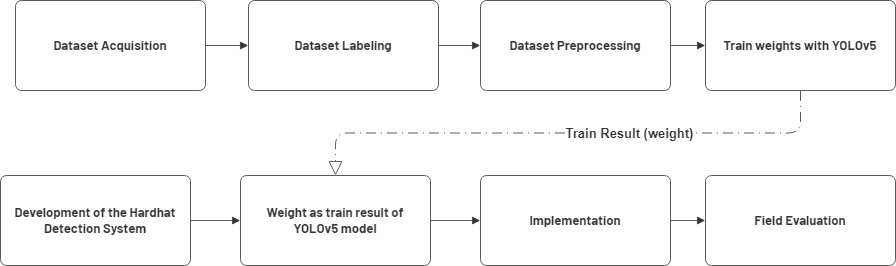
\includegraphics[width=0.9\textwidth]{gambar/utilities/methodologi_hardhat.png}

  \caption{Hardhat Detection using CNN Methodology}
  \label{fig:hedec_method}
\end{figure*}

\subsection{Dataset Acquisition}
\label{subsec:DatasetAcquisition}

\par The dataset used for training using Yolov5 is in the form of a dataset containing images containing field personnel who are wearing helmets and those who are not wearing helmets. For this study, the dataset used came from two sources, namely:

\begin{enumerate}
  \item Safety Helmet Detection by andrewmvd
  \par This dataset contains 5000 images of construction workers which including people who wear helmets and those who do not.  Each image has been labeled "helmet" and "head". The label annotation format is in the PASCAL VOC format which is stored in a .xml file. Sample of the this dataset are shown in Figure~\ref{fig:datasethelmetdetectionpreview}

  \begin{figure}[ht]
    \centering
    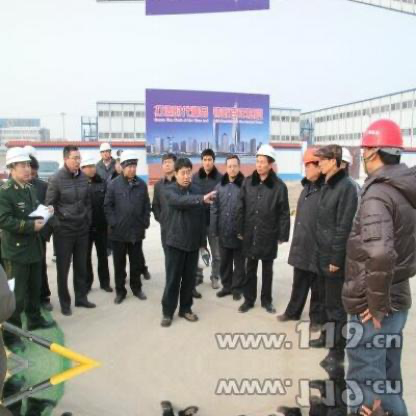
\includegraphics[width=0.24\textwidth]{gambar/sample_kaggle1/hard_hat_workers0.png}
    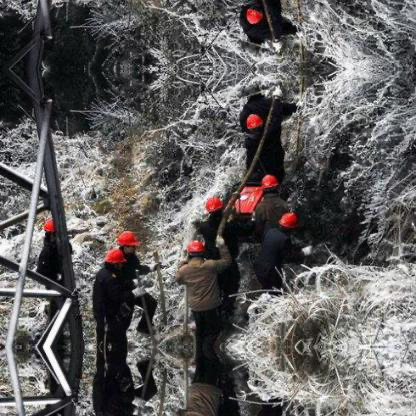
\includegraphics[width=0.24\textwidth]{gambar/sample_kaggle1/hard_hat_workers1.png}
    \caption{Dataset \emph{Safety Helmet Detection} by andrewmvd}
    \label{fig:datasethelmetdetectionpreview}  
  \end{figure}

  \item SampleERASTY2020 dataset by Alif Aditya Wicaksono
  \par This dataset contains 8,867 images whose content is similar to the previous Safety Helmet Detection dataset by andrewmvd. This dataset is also complete with annotations but requires some changes to suit the training method. In addition, the 8,867 images also include augmentation results such as flip, rotation, blur, and noise. Sample of the this dataset are shown in Figure~\ref{fig:dataseterastypreview}

  \begin{figure}[ht]
    \centering
    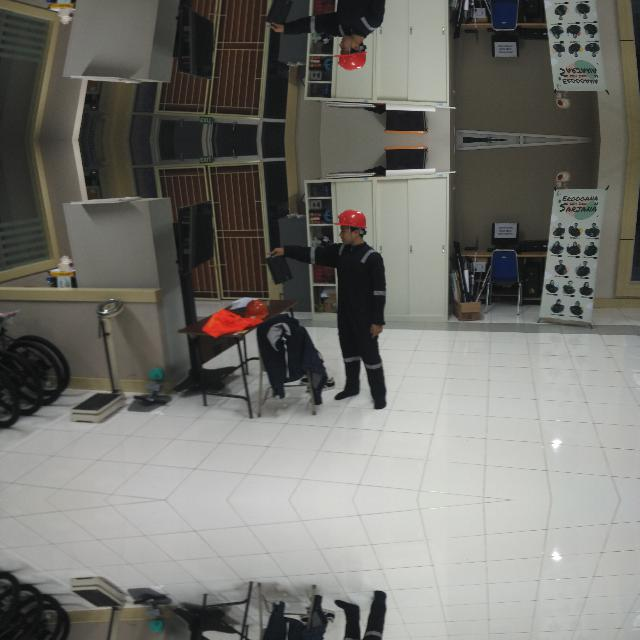
\includegraphics[width=0.24\textwidth]{gambar/sample_erasty/APB-Hat-6-_jpg.rf.79aa17f23c1834efa681edc7aca5cd5f.jpg}
    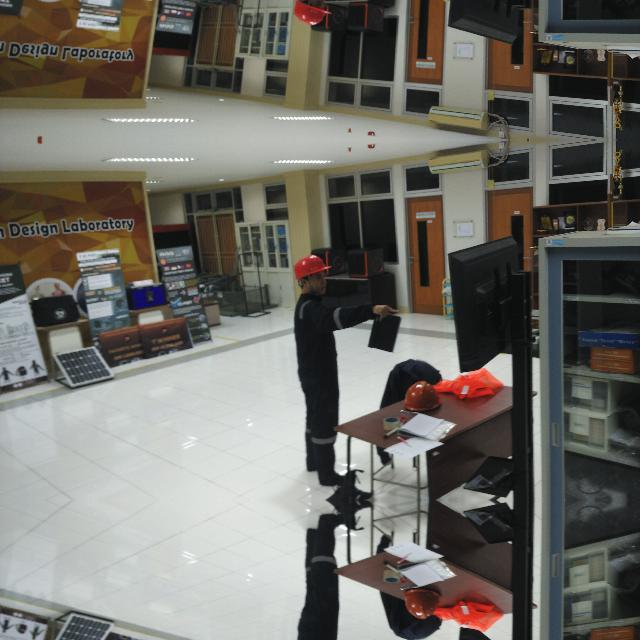
\includegraphics[width=0.24\textwidth]{gambar/sample_erasty/APB-Hat-7-_jpg.rf.4e9ff94579f598546de38a9b5c88a05d.jpg}
    \caption{Dataset SampleERASTY2020 by Alif Aditya Wicaksono}
    \label{fig:dataseterastypreview}  
  \end{figure}

\end{enumerate}

\subsection{Dataset Labeling}
\label{subsec:dataset_labeling}

\par The datasets that have been collected previously in Subsection~\ref{subsec:DatasetAcquisition} need to have annotations before being used as a training dataset. There are two classes used for this system :

\begin{enumerate}[nolistsep]
  \item "with\_helmet" which includes the head and the hardhat
  \item “no\_helmet” which includes the head without the hardhat
\end{enumerate}

\par The dataset that has been obtained already has its own labeling or annotation, but specifically for the SampleERASTY2020 dataset, there is an incompatibility for the Hard-hat label which only includes work safety helmets without the wearer's head. Therefore, a re-labeling of the SampleERASTY2020 dataset was carried out, which only used an image file that had not yet been augmented, totaling 338 images. The image labeling process is carried out on the Roboflow platform as shown in Figure~\ref{fig:gambarbesertalabel}.

\begin{figure}[ht]
  \centering
  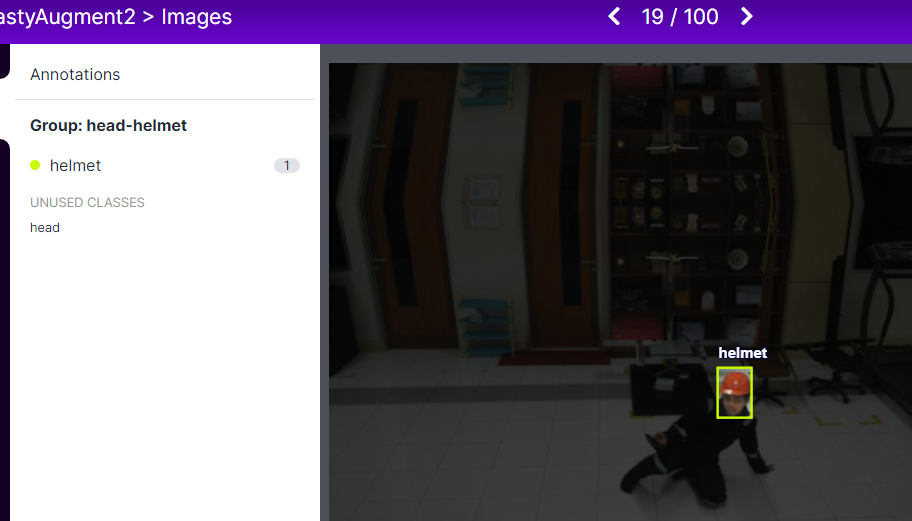
\includegraphics[width=0.4\textwidth]{gambar/utilities/labeldiroboflow.png}
  \caption{Image Labeling in Roboflow}
  \label{fig:gambarbesertalabel}  
\end{figure}

\subsection{Dataset Preprocessing}
\label{subsec:dataset_preprocessing}

\par Several processes are carried out for the datasets that have been collected so that they can be used for the training process properly. The process includes image resizing or resizing, renaming class names, and augmentation. For this research, these processes are carried out on the Roboflow platform.

\subsubsection{Image Resizing}
\label{subsec:imageresize}
\par YOLOv5 which is used to train the dataset accepts images in size 640x640 with RGB colors so the existing dataset will be resized to that size. The YOLOv5 source code from the GitHub repository already provides a resize feature before being trained but in order to preserve the image quality, the resizing process are being carried out using the Roboflow platform. 

\subsubsection{Dataset Cleanup}
\label{subsec:datasetcleanup}
\par Some images are not needed from the dataset obtained such as images that only have a safety vest which is not used for training purposes. Some of these images will not be included in the export dataset from roboflow.

\subsubsection{Class Rename}
\label{subsec:classrename}
\par The existing label class naming of the existing dataset will be adapted for easier use and understanding. The sampleERASTY2020 dataset that has been re-labeled does not need to go through this process, but the Safety Helmet Detection dataset needs to be renamed where for the “helmet” class it becomes “with\_helmet” and “head” becomes “no\_helmet” as shown in Figure \ref{fig:prepro_classrename}.

\begin{figure}[ht]
  \centering
  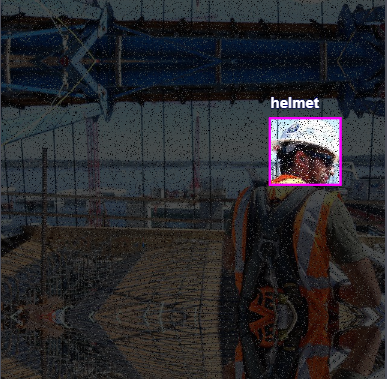
\includegraphics[width=0.24\textwidth]{gambar/utilities/reclass_old.png}
  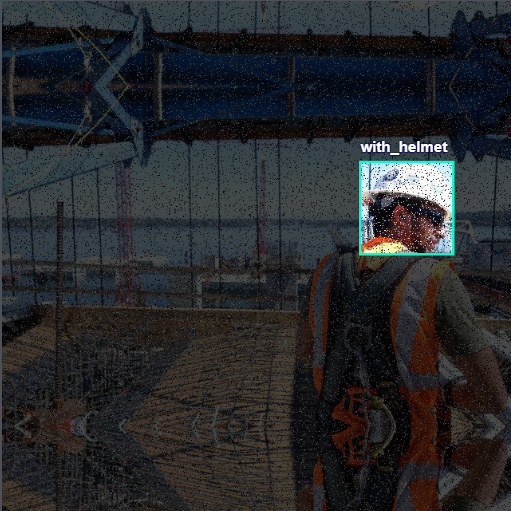
\includegraphics[width=0.24\textwidth]{gambar/utilities/reclass_new.png}
  \caption{Class Rename in Roboflow}
  \label{fig:prepro_classrename}  
\end{figure}

\subsubsection{Augmentation}
\label{subsec:augmentation}
\par Additional augmentation is also carried out on the dataset to add variations to the image in the dataset where the augmentation forms used are noise and horizontal flip as shown in Figure~\ref{fig:prepro_augmentasi}. The augmentation process is carried out on the Roboflow platform which also provides augmentation features. The re-labeled and additional augmented SampleERASTY2020 dataset was then combined with the previously obtained dataset of 5000 images of the Safety Helmet Dataset by andrewvmd.

\begin{figure}[ht]
  \centering
  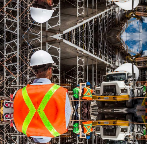
\includegraphics[width=0.24\textwidth]{gambar/utilities/aug_flip.png}
  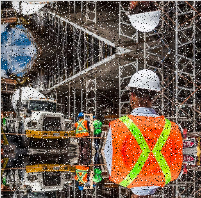
\includegraphics[width=0.24\textwidth]{gambar/utilities/aug_noise.png}
  \caption{\emph{Flip} and \emph{Noise} Augmentation}
  \label{fig:prepro_augmentasi}  
\end{figure}

\subsubsection{Dataset Subset}
\label{subsec:datasetsubset}
\par Before being used for weight training, the previously combined dataset needs to be divided into the train - test - val set. The division for the dataset used for training is 70\% train (4202) , 20\% test (1,200 images), and 10\% validation (600 images). For training using PyTorch-based YOLOv5, Roboflow provides an export dataset feature to a specified format where here the annotations are saved in the form of '.txt' and managed via a '.yaml' file. The distribution of this dataset is done through the Generate Dataset Version feature on the Roboflow platform. The dataset was obtained from the dataset merging process mentioned in Subsection~\ref{subsec:DatasetAcquisition} and after going through pre-processing.

\subsection{Training}
\label{subsec:dataset_training}

\par Datasets that have been pre-processed previously in roboflow and already have appropriate annotations are then used for training using YOLOv5. This training is a model training process with input images from annotated datasets where the images and annotations are processed to produce a special characteristic or pattern from a predetermined class/label through annotations so that the computer can then use the computer to guess the image that will be detected. . Especially for YOLOv5 which uses PyTorch as its machine learning framework, the training results in the form of weights will be exported in the form of '.pt' (pytorch format).

\begin{table} [ht]
  \caption{Train Configuration}
  \label{tb:trainconfig}
  \centering
  \begin{tabular}{|c|c|}
    \hline
    % \rowcolor[HTML]{C0C0C0}
    \textbf{Parameters} & \textbf{Detail}  \\
    \hline
    \emph{batch\textunderscore size} & 16 \\
    \emph{epoch} & 150 \\
    \emph{imgsize} & 640\\
    % \emph{data} & /content/yolov5/helmetDetection\textunderscore yolov5\textunderscore 2/data.yaml\\
    \emph{optimizer} & SGD (DEFAULT)\\
    \emph{device} & CUDA\\  
    \hline
  \end{tabular}
\end{table}

\par As can be seen in Table~\ref{tb:trainconfig}, the training process is carried out with batch sizes of 16 and 150 epochs with the default optimizer for yolov5 which is SGD. Batch\textunderscore size here determines the number of images that will be used to train in one iteration, determined 16 by considering the hardware limitations used for this training process. The training process is carried out in Colab Pro were with the given GPU Ram limitation, it is used up to 12 GB. For the image size itself, the algorithm provided by YOLOv5 only provides a 1:1 resolution whereby specifying the imgsize parameter 640 means the size for (height) and (width) becomes 640x640.

\par The training process in this research is carried out by utilizing pretrained weights provided from the YOLOv5 repository and also without using these pretrained weights with the aim of comparing the performance of the weights generated from these methods but will use a configuration similar to the configuration used to -train the pretrained weights. The weight variants that will be used are yolov5n (Nano), yolov5s (Small), yolov5m (Medium), and yolov5l (Large) variants. Based on the explanation from the YOLOv5 repository, the pretrained weights provided are the result of training using the COCO val2017 dataset parameter 300 epoch \cite{glenn_jocher_yolov5}. The main difference between these pretrained weights is in the "depth\_multiplier" and "width\_multiplier" parameters which have an impact on the layer depth and the number of channels of output for each layer. The nominal configuration of "depth\_multiplier" and "width\_multiplier" for each variant can be seen in the table.

\begin{table} [ht]
  \caption{depth\_multiplier and width\_muliplier Difference}
  \label{tb:pretrainedparamdiff}
  \centering
  \begin{tabular}{|l|l|l|}
    \hline
    \multirow{2}{*}{Model Name} & \multicolumn{2}{l|}{Multiplier}      \\ 
    \cline{2-3}
                                 & depth\_multiplier & width\_muliplier  \\ 
    \hline
    yolov5n\textit{ (Nano)}      & 0.33              & 0.25              \\
    yolov5s\textit{ (Small)}     & 0.33              & 0.5               \\
    yolov5m\textit{ (Medium)}    & 0.67              & 0.75              \\
    yolov5l\textit{ (Large)}     & 1                 & 1                 \\
    \hline
  \end{tabular}
\end{table}

\par The training process for this title is not carried out with local computer hardware but uses Google Colab Pro where the training process is run in the cloud. The previously collected dataset is downloaded to the Colab Pro vm storage directly from Roboflow. With limitations on the use of storage, ram, and GPU ram as well as runtime provided by Google Colab, checkpoints are stored for each training epoch on the author's drive. This is done for the possibility that in the middle of the VM Colab Pro training session, the VM Colab Pro terminates automatically on itself. 

\subsection{Development of The Hardhat Detection System}
\label{subsec:perancangansistemdeteksihelmkeselamatankerja}

\par This hardhat detection system will utilize YOLOv5 to make predictions on the input received. Input is an image received from a webcam or camera connected to a computer that will run this system. The system was developed with the aim of detecting the use of work safety helmets in real-time and will run an alarm mechanism if on the camera input there is someone who is not wearing a work safety helmet. The flowchart for the Safety Helmet Detection system can be seen at Figure~\ref{fig:flowchart_sistem}.

\par The system will be created as a python script file that can be run and can accept several parameters: input source, weight to be used, confidence threshold, and IoU threshold for the Non Max Suppression process.

\par Input that can be used with the created script can be done in the form of video files or camera feeds. The system can accept various resolutions, but for the inference process, the input dimensions will be resized to 640x640 and the output will be adjusted to the dimensions of the initial input.

\par Each frame that comes in from the input webcam will be used to process inference via
yolov5 model with weight that has been created previously through the training process.
The result of inference using YOLOv5 will return the input in the form of position for
the detected object is in xcenter, ycenter and the dimension of the object is in widht
and height as well as the name information class and confidence score for
each detected object. The result of output inference obtained is then used to draw
bounding box on the frame image being inference
as in Figure~\ref{fig:bboxresult}.

% Contoh input gambar pada kolom.
\begin{figure} [ht]
  \centering
  % Ubah sesuai dengan nama file gambar dan ukuran yang akan digunakan.
  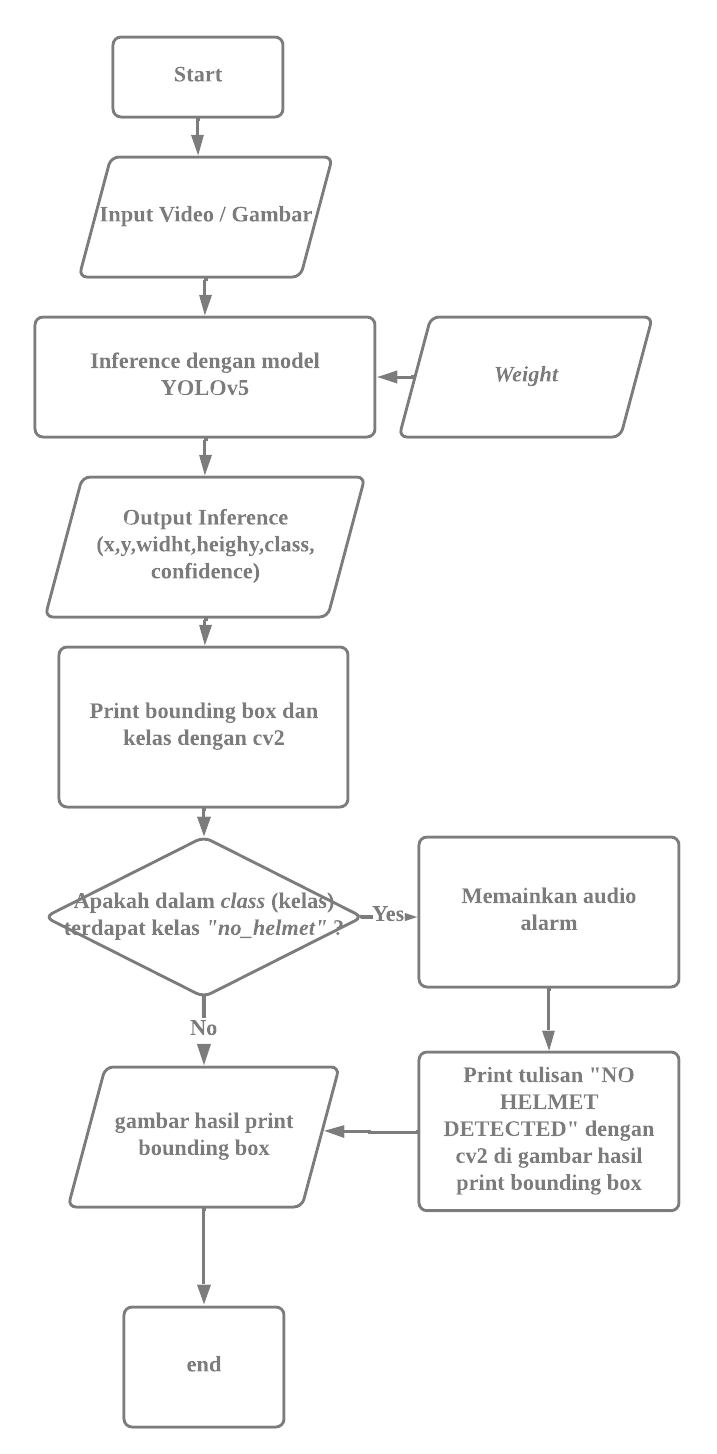
\includegraphics[width=0.4\textwidth]{gambar/flowchart_sistem.png}

  % Ubah sesuai dengan keterangan gambar yang diinginkan.
  \caption{Hardhat Detection System Flowchart}
  \label{fig:flowchart_sistem}
\end{figure}

\begin{figure} [ht]
  \centering
  % Ubah sesuai dengan nama file gambar dan ukuran yang akan digunakan.
  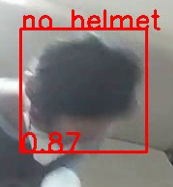
\includegraphics[width=0.2\textwidth]{gambar/utilities/bbox1.png}
  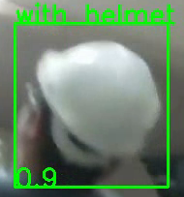
\includegraphics[width=0.2\textwidth]{gambar/utilities/bbox2.png}

  % Ubah sesuai dengan keterangan gambar yang diinginkan.
  \caption{Bounding Box Result}
  \label{fig:bboxresult}
\end{figure}


\par The alarm function will be executed when one or more 'no\_helmet' 
class object is detected inside the frame that is being \emph{inferenced} by the model. 
This alarm function contains commands to play the alarm audio to simulate a siren alarm. 
In addition to running the alarm function, it will also run a command to display 
“NO\_HELMET DETECTED” on the predicted frame as shown in Figure~\ref{fig:alarmtriggerexample}.

\begin{figure} [ht]
  \centering
  % Ubah sesuai dengan nama file gambar dan ukuran yang akan digunakan.
  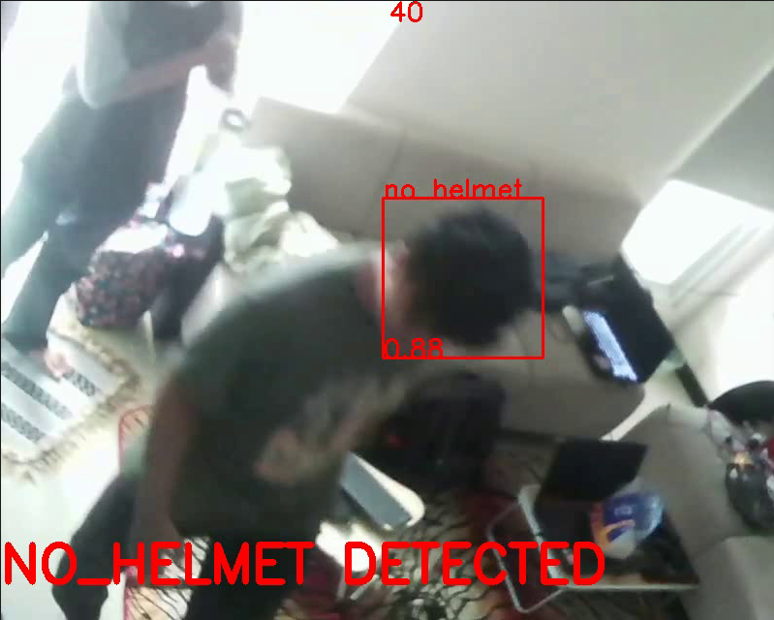
\includegraphics[width=0.4\textwidth]{gambar/utilities/alarm_example.png}

  % Ubah sesuai dengan keterangan gambar yang diinginkan.
  \caption{Example On Alarm Trigger}
  \label{fig:alarmtriggerexample}
\end{figure}

\par As an addition, the Frame-rate counter will be shown on the middle top of the window 
of the output. This is done as a way to benchmark the performance of each model that 
is being tested in this research where YOLOv5 provides a Small variant to a Large variant. 
It is expected the larger the model, the smaller the frame per second (FPS) will be.

\subsection{You Only Look Once (YOLO)}
\label{subsec:yolo_base}

\par You Only Look Once or YOLO is a very fast multi-object detection algorithm that was introduced by Redmond et al in 2015 through their book You Only Look Once: Unified, Real-Time Object Detection \cite{redmon2016you}. The Convolutional Neural Network (CNN) is the basis of this YOLO detection system. YOLO performs object detection by considering it as a single regression problem that is taken directly from the pixels in the image into a bounding box marker of coordinates and probability of classification. That way it only needs to be checked once on the image to detect or identify. \cite{redmon2016you} YOLO combines several components of the object text into a single neural network that uses features from all parts of the image to predict each bounding box while simultaneously predicting all bounding boxes in all types of classifications. The design of YOLO allows for end-to-end training and real-time detection speed.

\par The YOLO system itself divides the input image into an S x S grid. The role of the grid here is for later, that is, if a certain grid becomes the center of the object, then that grid will be useful for detecting the object earlier.

\par Each grid predicts each bound box and the value of the possible classification or confidence score of the bounding box. This value represents how "sure" the model is of the object detected in the bounding box and how accurate its prediction is.

\par There are five predicted values in each bounding box, namely: x, y, w, h, and confidence. X and Y represent the center of the bounding box. W and H represent the relative predicted Weight and Height of the entire image. Then the confidence score itself represents the IOU between the predicted box and the ground truth box \cite{redmon2016you}.

\subsubsection{YOLOv5}
\label{subsecsec:yolov5}

\par YOLOv5 is an updated version of YOLO which was created in 2020 by Glenn Jocher \cite{glenn_jocher_yolov5}. Based on the Github repository for YOLOv5 by Glenn Jocher, the network structure of YOLOv5 is divided into 3 main parts, namely Backbone, Neck, and Head modules. As can be seen in Figure \ref{fig:yolov5network}. 

\par The network structure of YOLOv5 starts from the Backbone module where the input image is passed first to extract features from the image whose structure is based on CSP-Darknet53. But before going through the Backbone, the input image are being pass through the Focus structure. Inside the backbone, the input go through several  Bottleneck CSP Networks (Cross Stage Partial Networks) and then  and Spatial Pyramid Pooling (SPP). The main purpose of the Spatial Pyramid Pooling block is to generate output with the same size regardless of the size of the input frame. The result of feature extraction from Backbone is then used to generate \emph{feature pyramid} in the Neck module which is a structure based on PANet (Path Aggregation Network). Finally, in the Head Module, the information needed to draw bounding box and to tell what class is being detected is generated here which includes some information, namely: class, coordinates, and confidence score.

\begin{figure*} [ht]
  \centering
  % Ubah sesuai dengan nama file gambar dan ukuran yang akan digunakan.
  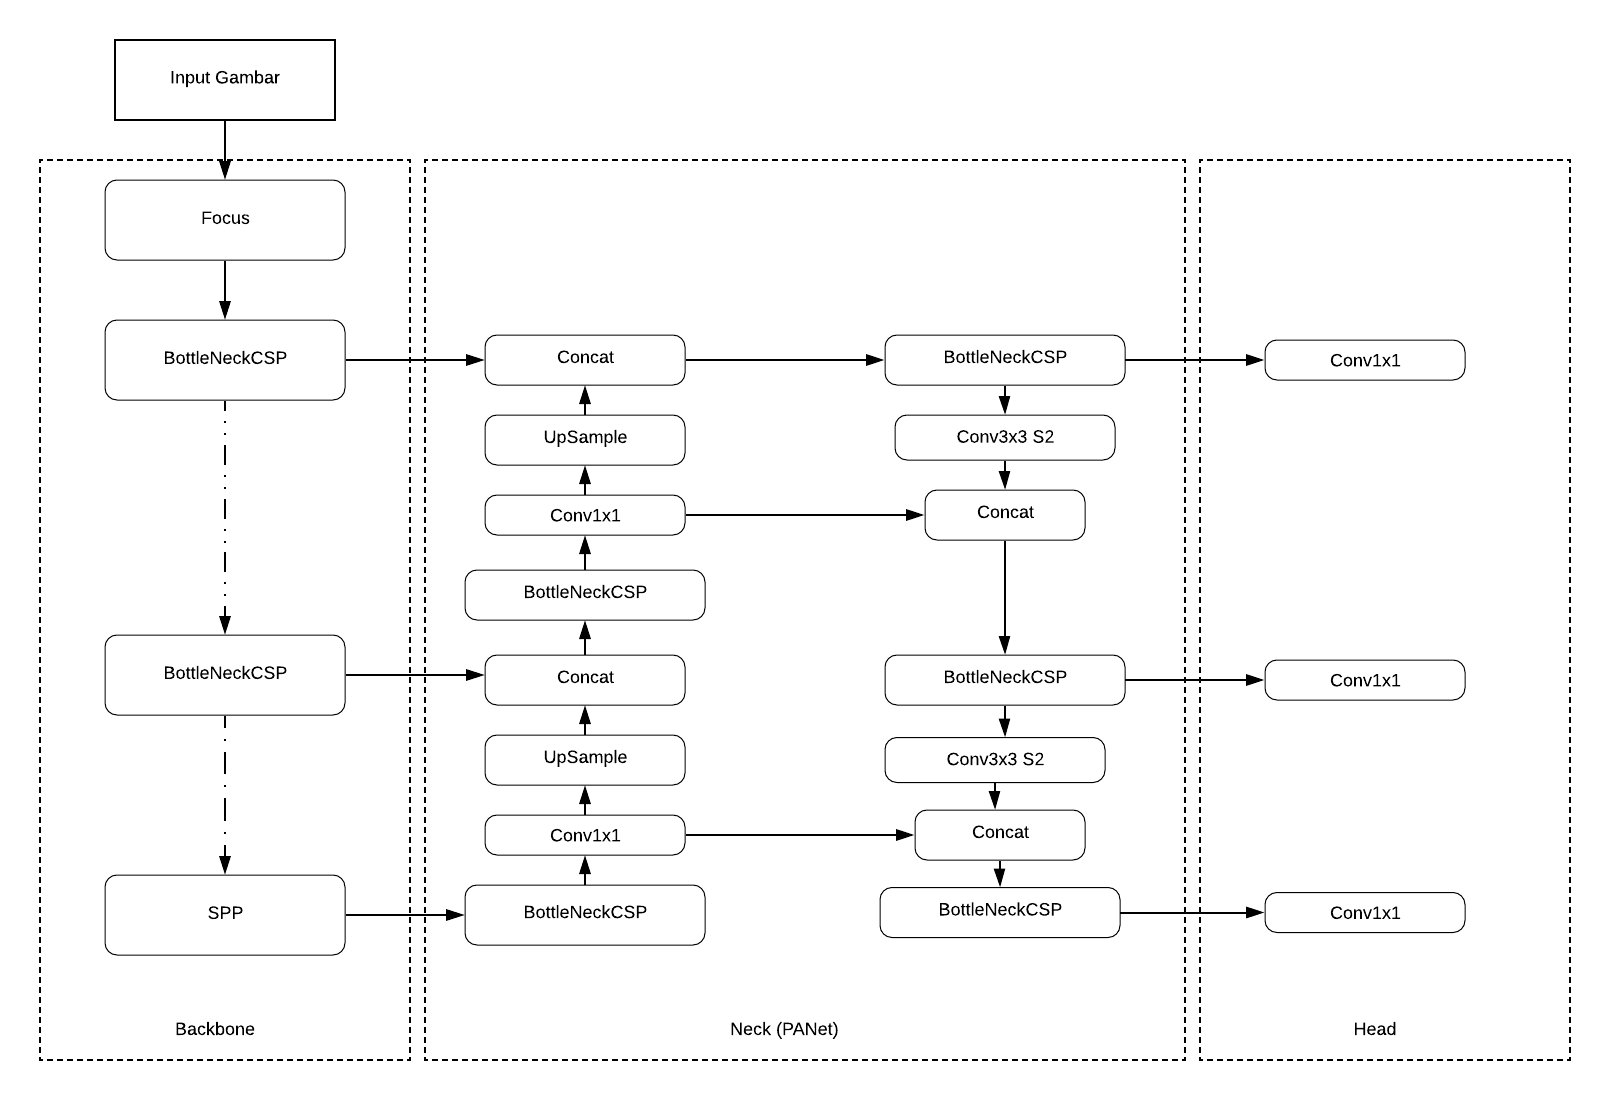
\includegraphics[width=0.9\textwidth]{gambar/yolov5 structure.png}

  % Ubah sesuai dengan keterangan gambar yang diinginkan.
  \caption{YOLOv5 Network}
  \label{fig:yolov5network}
\end{figure*}
  % Ubah judul dan label berikut sesuai dengan yang diinginkan.
\section{Results and Analysis}
\label{sec:resultnanalysis}

\par Bab ini akan membahas hasil dan analisa dari desain sistem yang sudah dibuat dan implementasinya. Pengujian terhadap hasil dibagi menjadi beberapa bagian.

\subsection{Pengujian Performa antar \emph{Weight}}
\label{subsec:modeltest}
% Ubah paragraf-paragraf pada bagian ini sesuai dengan yang diinginkan.

% \par The YOLOv5 repository provides several checkpoints or weights that result from training the YOLOv5 model from the COCO dataset used as a pre-trained model. The expectation of using this pre-trained model is that the resulting weight will perform better than doing training without any pretrained model. This COCO dataset has 80 different classes. However, as mentioned in \ref{subsec:dataset_labeling}, this research, only requires 2 classes, namely "no\_helmet" and "with\_helmet".

\par Repositori YOLOv5 menyediakan beberapa \emph{checkpoint} atau \emph{weight} yang merupakan hasil training model YOLOv5 dari dataset COCO yang dimanfaatkan sebagai \emph{pretrained model}. Ekspektasi penggunaan pretrained model ini yaitu bobot yang dihasilkan akan memiliki performa yang lebih tinggi daripada melakukan training tanpa pretrained model sama sekali. \emph{COCO Dataset} ini memiliki 80 \emph{class} berbeda. Seperti disebutkan pada \ref{subsec:dataset_labeling} yaitu untuk keperluan penelitian ini hanya memerlukan 2 kelas yaitu "no\textunderscore helmet" dan "with\textunderscore helmet".

% \par Some of the pre-trained models provided from the YOLOv5 repository are YOLOv5n, YOLOV5s, YOLOv5m, YOLOv5l, YOLOv5l, and YOLOv5x. In addition to these pre-trained models, there is also a version for the 1280 image size, namely the YOLOv5n6 to YOLOv5l6 series. In this study, only the YOLOv5n to YOLOv5l variations are used because the YOLOv5x variation and the 6 series version for 1280 image sizes take longer. The differences in the pre-trained weights stem from the initial configuration of training on the COCO dataset using YOLOv5, especially the "depth\_multiple" and "width\_multiple" parameters.

\par Beberapa \emph{pretrained model} yang disedikana dari repositori YOLOv5 yaitu YOLOv5n, YOLOV5s, YOLOv5m, YOLOv5l,YOLOv5l, dan YOLOv5x. Selain beberapa model pretrained tersebut juga ada versi untuk ukuran gammbar 1280 yaitu seri YOLOv5n6 hingga YOLOv5l6. Pada penelitian ini hanya menggunakan variasi YOLOv5n hingga YOLOv5l karena variasi YOLOv5x dan versi seri 6 untuk ukuran gambar 1280 membutuhkan waktu yang lebih lama. Perbedaan - perbedaan yang ada pada bobot - bobot pretrained tersebut berasal dari konfigurasi awal dari training pada dataset COCO yang menggunakan YOLOv5, terutama pada paramter "depth\textunderscore multiple" dan "width\textunderscore multiple".

% \par The validation process of the training results is carried out using the Safety Helmet Detection dataset, whose distribution is described in the \ref{subsec:dataset_preprocessing} section, which consists of 1200 images with the "no\_helmet" class totalling 1322 labels and the "with\_helmet" class totalling 4294 labels.

\par Proses validasi hasil training dilakukan menggunakan dataset Deteksi Helm Keselamatan Kerja yang pembagiannya dijelaskan pada bagian \ref{subsec:dataset_preprocessing} yang berjumlah 1200 gambar dengan kelas "no\textunderscore helmet" berjumlah 1322 label dan kelas "with\textunderscore helmet" berjumlah 4294 label.

% \par In this section, we will compare the performance of each weight generated with the pre-trained model and those without the pre-trained model. This test was carried out using resources from Google Colab. The Google Colab resource specifications used when validating for weights that have been {trained} can be seen in Table~\ref{tb:spekgoogleclab}.

\par Pada bagian ini akan dipaparkan dan dibandingkan performa antara tiap bobot yang dihasilkan dengan model pretrained dan yang tidak menggunakan pretrained model. Pengujian ini dilakukan menggunakan \emph{resource} dari Google Colab. Spesifikasi \emph{resource} Google Colab yang digunakan saat melakukan validasi untuk bobot yang sudah di-\emph{train} dapat dilihat pada Tabel~\ref{tb:spekgoogleclab}.

\begin{table}
  \centering
  \caption{Spesifikasi \emph{Resource} Google Colab Untuk Validasi \emph{Weight}}
  \label{tb:spekgoogleclab}
  \begin{tabular}{|l|l|} 
  \hline
  Type    & Detail                      \\ 
  \hline
  Python  & Python-3.7.13                   \\
  PyTorch & torch-1.11.0+cu113              \\
  GPU     & Tesla P100-PCIE-16GB, 16281MiB  \\
  \hline
  \end{tabular}
\end{table}

\begin{table*}
  \centering
  \caption{Pretrained Model Peformance Test Result}
  \label{tb:pretrainbenchmarktest}
  \begin{tabular}{|l|l|l|l|l|l|l||} 
    \hline
    Weight Name                          & class        & precision & recall & mAP   & mAP .5:.95 & inference time (ms)    \\ 
    \hline
    \multirow{3}{*}{hedec\_pretrain\_N} & all          & 0.925     & 0.871  & 0.922 & 0.557      & \multirow{3}{*}{1.9}   \\
                                        & no\_helmet   & 0.924     & 0.867  & 0.916 & 0.552      &                        \\
                                        & with\_helmet & 0.926     & 0.875  & 0.929 & 0.562      &                        \\ 
    \hline
    \multirow{3}{*}{hedec\_pretrain\_S} & all          & 0.929     & 0.878  & 0.929 & 0.568      & \multirow{3}{*}{4}     \\
                                        & no\_helmet   & 0.925     & 0.857  & 0.918 & 0.561      &                        \\
                                        & with\_helmet & 0.932     & 0.9    & 0.941 & 0.575      &                        \\ 
    \hline
    \multirow{3}{*}{hedec\_pretrain\_M} & all          & 0.923     & 0.891  & 0.933 & 0.57       & \multirow{3}{*}{8.7}   \\
                                        & no\_helmet   & 0.919     & 0.883  & 0.923 & 0.561      &                        \\
                                        & with\_helmet & 0.928     & 0.898  & 0.943 & 0.58       &                        \\ 
    \hline
    \multirow{3}{*}{hedec\_pretrain\_L} & all          & 0.919     & 0.867  & 0.919 & 0.579      & \multirow{3}{*}{14}    \\
                                        & no\_helmet   & 0.904     & 0.846  & 0.899 & 0.565      &                        \\
                                        & with\_helmet & 0.934     & 0.887  & 0.939 & 0.593      &                        \\ 
    \hline
  \end{tabular}
\end{table*}

% \par Based on the validation results presented, there is no significant difference in precision, recall, mAP@.5 in either the "with\_helmet" or "no\_helmet" classes, as shown in Figure~\ref{tb:pretrainbenchmarktest}. The precision value is above 0.9, with the highest value being the "hedec\_pretrain\_S" variant. The recall is also not too different between the weights where everything is above the number 0.8, with the highest value being the "hedec\_pretrain\_M" variant.

\par Berdasarkan hasil validasi yang dipaparkan, tidak ada perbedaan signifikan dari \emph{precision, recall, mAP} 
baik pada kelas "with\_helmet" ataupun "no\_helmet" seperti yang ditunjukan pada Tabel~\ref{tb:pretrainbenchmarktest}.
Untuk nilai \emph{precision} berada di atas 0.9 dengan nilai tertinggi oleh varian "hedec\_pretrain\_S" . Untuk \emph{recall}
juga tidak terlalu berbeda diantara bobot dimana semuanya berada diatas angka 0.8 dengan bilai teringgi 
oleh varian "hedec\_pretrain\_M". 


\begin{table*}
  \centering
  \caption{Model Without Pretrained Test Result}
  \label{tb:purebenchmarktest}
  \begin{tabular}{|l|l|l|l|l|l|l||} 
    \hline
    Weight Name                          & class        & precision & recall & mAP   & mAP .5:.95 & inference time (ms)    \\ 
    \hline
    \multirow{3}{*}{hedec\_pure\_N}     & all          & 0.918     & 0.848  & 0.909 & 0.532      & \multirow{3}{*}{1.9}   \\
                                        & no\_helmet   & 0.919     & 0.839  & 0.903 & 0.52       &                        \\
                                        & with\_helmet & 0.918     & 0.856  & 0.915 & 0.544      &                        \\ 
    \hline
    \multirow{3}{*}{hedec\_pure\_S}     & all          & 0.926     & 0.866  & 0.919 & 0.555      & \multirow{3}{*}{4.2}   \\
                                        & no\_helmet   & 0.925     & 0.86   & 0.911 & 0.55       &                        \\
                                        & with\_helmet & 0.927     & 0.872  & 0.927 & 0.559      &                        \\ 
    \hline
    \multirow{3}{*}{hedec\_pure\_M}     & all          & 0.932     & 0.866  & 0.924 & 0.564      & \multirow{3}{*}{8.9}   \\
                                        & no\_helmet   & 0.937     & 0.856  & 0.917 & 0.562      &                        \\
                                        & with\_helmet & 0.927     & 0.877  & 0.93  & 0.566      &                        \\ 
    \hline
    \multirow{3}{*}{hedec\_pure\_L}     & all          & 0.922     & 0.876  & 0.923 & 0.566      & \multirow{3}{*}{14.1}  \\
                                        & no\_helmet   & 0.919     & 0.868  & 0.914 & 0.561      &                        \\
                                        & with\_helmet & 0.925     & 0.884  & 0.932 & 0.572      &                        \\
    \hline
  \end{tabular}
\end{table*}

% \par Based on the validation results carried out for the weights that were trained without using Pretrained Weights from YOLOv5, several conclusions are concluded. As can be seen Figure~\ref{tb:purebenchmarktest} for the average of all classes , for precision generally above 0.9 and recall above 0.8, as well as mAP.5 which is above 0.9. But in terms of inference time for each variant, there is not much difference when compared weights are trained using Pretrained Weights from YOLOv5.

\par Berdasarkan hasil validasi yang dilakukan untuk bobot - bobot yang dilatih tanpa menggunakan \emph{Pretrained Weights} dari YOLOv5 yang dapat ditarik beberapa point.Seperti yang dapat dilihat pada Tabel~\ref{tb:purebenchmarktest}, untuk masing-masing kelas, ntuk \emph{precision} secara umum berada di atas 0.9 dan \emph{recall} di atas 0.8, begitu juga dengan mAP.5 nya yang berada ditas 0.9. Tetapi dari segi \emph{inference time} untuk masing - masin varian, tidak ada perbedaan jauh jika dibandingkan bobot - bobot yang di latih menggunakan \emph{Pretrained Weights}.

\subsection{Pengujian Performa Berdasarkan Jarak}
\label{subsec:model_rangetest}

\par Pada bagian ini akan memaparkan hasil deteksi pada dataset validasi yang dibagi menjadi beberapa variasi jarak dari kamera. Dataset yang digunakan meliputi 8 foto untuk jarak 1,3 meter hingga 9 meter. Hasil pengujian ini ditunjukan pada Gambar~\ref{fig:pretrain_dist_test} bobot yang di-\emph{train} menggunakan \emph{Pretrained Weights} dan  Gambar~\ref{fig:pure_dist_test} untuk bobot yang di-\emph{train} tanpa \emph{Pretrained Weights}.
 
\begin{figure}[ht]
  \centering
  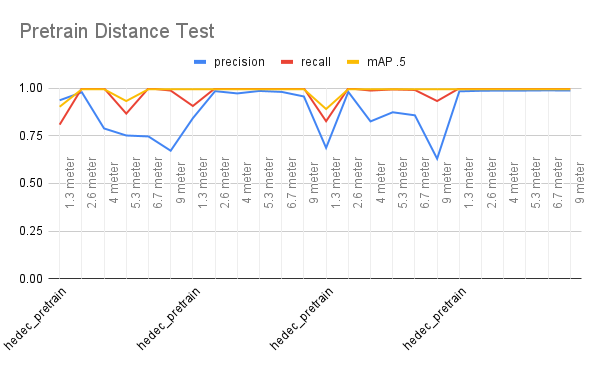
\includegraphics[width=0.4\textwidth]{gambar/utilities/pretain_dist_test.png}
  \caption{Pretrained Model Distance Difference Test}
  \label{fig:pretrain_dist_test}  
\end{figure}

\begin{figure}[ht]
  \centering
  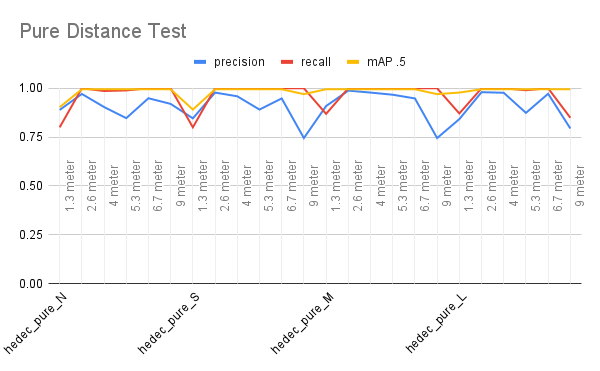
\includegraphics[width=0.4\textwidth]{gambar/utilities/pure_dist_test.png}
  \caption{Without Pretrained Model Distance Difference Test}
  \label{fig:pure_dist_test}  
\end{figure}

\subsection{Pengujian Pada Tingkat Kecerahan Rendah}
\label{subsec:model_lowillum_test}

% \par This section describes the model's performance in detecting low-brightness input images. The validation data contains 35 images with the number of labels no\textunderscore helmet 20 and labels with\textunderscore helmet 57. In addition, validation is carried out on the training results using pre-trained weight and those without pre-trained weight. The test conducted using all the available weight variants as show in Figure~\ref{fig:lowillum_test}.

\par Bagian ini memaparkan performa model melakukan
deteksi pada input gambar dengan tingkat kecerahan rendah. Data validasi berisi
35 gambar dengan jumlah label \emph{no\_helmet} 20 dan label \emph{with\_helmet} 57.
Validasi dilakukan pada bobot hasil training yang menggunakan \textit{pretrained weight} dan yang tanpa menggunakan \textit{pretrained weight}. Hasil pengujian ini ditunjukkan pada Gambar~\ref{fig:lowillum_test}.

\begin{figure}[ht]
  \centering
  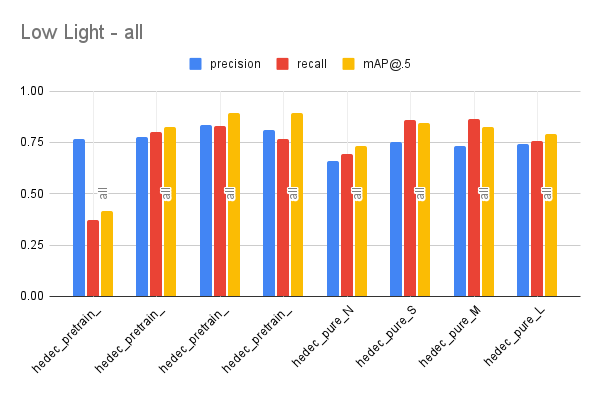
\includegraphics[width=0.4\textwidth]{gambar/utilities/lowlight_test.png}
  \caption{Pengujian Kecerahan Rendah}
  \label{fig:lowillum_test}  
\end{figure}

% \subsection{Frame Rate Test on Jetson Nano}
% \label{subsec:model_jetsonnano_test}

% \par This section is an explanation of the results of the YOLOv5 Model performance testing when being run on Jetson Nano with the weights that have been previously trained Nano. This test aims to compare the effectiveness of each weight that has been made on the inference performance aspect, considering that the Jetson Nano is a mini-computer with its own Graphics Processing Unit (GPU) and is designed for AI IoT applications. Therefore, the measurement taken in this test is the Frame Per Second (FPS) value.

 
% \par Tests were carried out using the Nemesis NYK A-90 Everest Webcam attached to the Jetson Nano via a USB cable. The tests were carried out at resolutions 256, 480, and 640. The results of the FPS measurement on the YOLOv5 Helmet Detection test are presented in Table~\ref{tb:jetsonano_model_benchmark}.

% \begin{table}
%   \centering
%   \caption{Jetson Nano Model Framerate Benchmark}
%   \label{tb:jetsonano_model_benchmark}
%   \begin{tabular}{|l|l|l|l|} 
%     \hline
%     \multirow{2}{*}{\textbf{Nama Bobot}} & \multicolumn{3}{l|}{\textbf{Resolusi}}      \\ 
%     \cline{2-4}
%                                          & \textbf{256} & \textbf{480} & \textbf{640}  \\ 
%     \hline
%     hedec\_pretrain\_N                   & 24.4         & 22           & 18.5          \\
%     hedec\_pretrain\_S                   & 22.2         & 13           & 7.8           \\
%     hedec\_pretrain\_M                   & 15.2         & 5.7          & 3.4           \\
%     hedec\_pretrain\_L                   & 8            & 3.2          & 1.8           \\
%     hedec\_pure\_N                       & 24.9         & 21.5         & 18.4          \\
%     hedec\_pure\_S                       & 23           & 12.3         & 7.8           \\
%     hedec\_pure\_M                       & 15           & 5.4          & 3.3           \\
%     hedec\_pure\_L                       & 8.3          & 3            & 1.8           \\
%     \hline
%   \end{tabular}
% \end{table}

\subsection{Pengujian Model YOLOv5 dengan \emph{Helmet Detection Weights} Pada Jetson Nano}
\label{sec:jetsonnano_hedectest}

\par Bagian ini merupakan pemaparan hasil pengujian performa Model YOLOv5 dengan bobot - bobot yang sudah di\emph{train}
sebelumnya pada Jetson Nano. Tujuan dari pengujian ini yaitu membandingkan effektifitas dari masing - masing
bobot yang sudah dibuat pada aspek performa \emph{inference} mengingat Jetson Nano merupakan \emph{mini-computer} yang memiliki
\emph{Graphic Processing Unit}(GPU)nya sendiri dan memang didesain untuk aplikasi AI IoT. Pengujuran yang diambil pada pengujian ini
yaitu nilai \emph{Frame Per Second}(FPS).

 
\par Pengujian dilakukan menggunakan Webcam Nemesis NYK A-90 Everest yang dipasang dengan Jetson Nano melalui kabel USB. 
Pengujian dilakukan pada resolusi 640. Hasil pengukuran FPS pada pengujian YOLOv5 Helmet Detection dipaparkan pada Tabel~\ref{tb:jetsonano_model_benchmark}.

\begin{table}
  \centering
  \caption{Jetson Nano Model Framerate Benchmark}
  \label{tb:jetsonano_model_benchmark}
  \begin{tabular}{|l|l|l|l|} 
    \hline
    \textbf{Nama Bobot} & \textbf{FPS}      \\ 
    \hline
    hedec\_pretrain\_N                             & 18.5          \\
    hedec\_pretrain\_S                             & 7.8           \\
    hedec\_pretrain\_M                           & 3.4           \\
    hedec\_pretrain\_L                            & 1.8           \\
    hedec\_pure\_N                              & 18.4          \\
    hedec\_pure\_S                              & 7.8           \\
    hedec\_pure\_M                              & 3.3           \\
    hedec\_pure\_L                                 & 1.8           \\
    \hline
  \end{tabular}
\end{table}


\subsection{Pengujian Sistem Deteksi Helm Keselamatan Kerja}
\label{subsec:hedect_sys_test}

% \par This subsection will display various tests on the helmet detection system. The workflow of the Hardhat Detection System is previously explained in Subsec~\ref{subsec:hedect_dev_sys} as also explained on there that the system will trigger an alarm in the form of a siren alarm when there is one or more "no\_helmet" class is detected within the frame.

\par Pada bagian ini akan dipaparkan berbagai macam pengujian terhadap sistem deteksi yang dikembangkan. Seperti yang sebelumnya sudah dijelaskan pada Subab~\ref{subsec:hedect_dev_sys}, sistem deteksi helm keselamatan kerja ini akan menjalankan mekanisme alarm berupa suara audio sirine alarm jika dalam frame terdeteksi satu atau lebih kelas "no\_helmet".

% \par The tests mostly are done by taking samples of frames from recorded system testing on various conditions: distance difference, low illuminance, CCTV angle, and Jetson Nano run. For this test, as it focuses on "How accurately the system fired the alarm when actually needed to", the "positive" is seen from when the alarm is triggered, and the "negative" are seen from when the alarm is not activated. The variant of weight used in these test is "hedec\_pretrain\_S".

\par Pengujian - pengujian sebagian besar dilakukan dengan cara mengambil beberapa sampel gambar dari hasil rekaman sistem di beberapa kondisi berbeda : perbedaan jarak, kecerahan rendah, sudut pandang CCTV, dan percobaan penjalanan di SBC Jetson Nano. Pengujian ini berfokus untuk menjawab pertanyaan "Seberapa akurat sistem menyalakan alarm saat alarm memang dibutuhkan untuk dinyalakan?". Sisi "Positif" akan dilihat dari saat alarm dinyalakan dan "Negatif" saat alarm tidak menyala. 

\subsubsection{Pengujain Sistem Pada Perbedaan jarak}
\label{subsubsec:hedect_test_dist}

% \par This test is conducted with the various distance between the camera and the object (person wearing and not wearing a hardhat) observed. The test is conducted by taking samples of frames from a predicted pre-recorded video with a person moving and rotating from 1 meter to 10 meters. The result of each distance variants are shown in Table~\ref{tb:systest_dist_test}.

\par Pengujian ini dilakukan dengan pada perbedaan jarak antara kamera dengan objek yang diamati (orang yang memakai atau tidak memakai helm keselamatan kerja). Pengujian dilakukan dengan mengambil beberapa sampel gambar dari rekaman yang menjalankan deteksi pada jarak 1 meter hingga 10 meter. Hasil pengujian dari masing - masing jarak ditunjukkan pada Tabel~\ref{tb:systest_dist_test}.

\begin{table}
  \centering
  \caption{System Test on Distance Difference}
  \label{tb:systest_dist_test}
  \begin{tabular}{|l|l|l|l|l|l|l|} 
  \hline
  Distance & TP & TN & FP & FN & Accuracy     & Samples of Test  \\ 
  \hline
  1m       & 17 & 61 & 7  & 0  & 0.9176470588 & 85               \\ 
  \hline
  3m       & 20 & 44 & 0  & 2  & 0.9696969697 & 66               \\ 
  \hline
  5m       & 40 & 53 & 0  & 0  & 1            & 93               \\ 
  \hline
  7m       & 32 & 56 & 0  & 0  & 1            & 88               \\ 
  \hline
  10m      & 78 & 32 & 0  & 0  & 1            & 110              \\
  \hline
  \end{tabular}
\end{table}


\subsubsection{Pengujian Pada Sudut Pandang CCTV}
\label{subsubsec:hedect_test_cctv}

% \par This test is conducted to imitate how CCTV is placed at a checkpoint on a construction site which usually is at a 45-degree angle. The test results are showin in Table~\ref{tb:systest_cctv}.

\par Pengujian ini dilakukan dengan tujuan mengimitasi bagaimana CCTV biasanya dipasang pada suatu \emph{checkpoint} di lokasi konstruksi yang biasanya dipasang dengan sudut 45 derajat. Hasil pengujian ini ditunjukan pada Tabel~\ref{tb:systest_cctv}.

\begin{table}
  \centering
  \caption{System Test on CCTV angle}
  \label{tb:systest_cctv}
  \begin{tabular}{|l|l|l|l|l|} 
  \hline
  TP & TN & FP & FN & Accuracy         \\ 
  \hline
  27 & 28 & 0  & 9  & 0.859375         \\ 
  \hline
  \multicolumn{2}{|l|}{55}   & \multicolumn{2}{l|}{9} & 64 test samples  \\
  \hline
  \end{tabular}
\end{table}


\subsubsection{Pengujian \emph{Real-Time} Pada Jetson Nano}
\label{subsubsec:hedect_test_cctv_jetsonanno}

% \par This test is also conducted to imitate how CCTV is placed at a checkpoint on a construction site, usually at a 45-degree angle. But the difference is that the system is being run in real-time. Unlike the other test where the prediction is being done on a pre-recorded video, in this test, the prediction is being run in real-time as the system actively detects using the webcam feeds. The test results are shown in Table~\ref{tb:systest_jetsonnano}.

\par Pengujian ini dilakukan dengan memanfaatkan Jetson Nano untuk \emph{deployment} dari sistem deteksi helm keselamatan kerja. Dengan menggunakan camera yang sama dan dipasang dengan sudut yang sama seperti pada Subbab~\ref{subsubsec:hedect_test_cctv} yang lalu dilakukan penjalanan sistem deteksi secara \emph{real-time}. Hasil rekaman penjalanan sistem lalu disimpan dan diambil sejumlah 33 sampel untuk pengujian yang ditunjukan pada Tabel~\ref{tb:systest_jetsonnano}.

\begin{table}
  \centering
  \caption{Hasil Pengujian \emph{Real-Time} Pada Jetson Nano}
  \label{tb:systest_jetsonnano}
  \begin{tabular}{|l|l|l|l|l|} 
  \hline
  TP & TN                    & FP & FN                & Accuracy         \\ 
  \hline
  14 & 17                    & 0  & 2                 & 0.9393939394     \\ 
  \hline
  \multicolumn{2}{|l|}{31}   & \multicolumn{2}{l|}{2} & 33 test samples  \\
  \hline
  \end{tabular}
\end{table}

\subsubsection{Pengujian Sistem Pada Keadaan Rendah Cahaya (Sore)}
\label{subsubsec:hedect_test_lowillum_dusk}

% \par This test is also conducted at a dusk time when illuminance is fairly low, and the sky is still lit. The test result is shown on Table~\ref{tb:systest_lowillum_dusk}. For this test there is 75 samples of test.

\par Pengujian ini juga dilakukan pada waktu senja ketika penerangan cukup rendah, dan langit masih terang. Hasil pengujian dapat dilihat pada Tabel~\ref{tb:systest_lowillum_dusk}. Untuk pengujian ini terdapat 75 sampel pengujian.


\begin{table}
  \centering
  \caption{System Test in Low Illuminance (Dusk)}
  \label{tb:systest_lowillum_dusk}
  \begin{tabular}{|l|l|l|l|l|} 
  \hline
  TP & TN                    & FP & FN                & accuracy         \\ 
  \hline
  45 & 25                    & 0  & 5                 & 0.9333333333    \\ 
  \hline
  \multicolumn{2}{|l|}{31}   & \multicolumn{2}{l|}{2} & 33 test samples  \\
  \hline
  \end{tabular}
\end{table}

\subsubsection{Pengujian Sistem Pada Keadaan Rendah Cahaya (Malam)}
\label{subsubsec:hedect_test_lowillum_dark}

% \par This test is also conducted at a dusk time when illuminance is very low with only one light source. The test result is shown on Table~\ref{tb:systest_lowillum_dark}. For this test there is 250 samples of test.

\par Tes ini juga dilakukan pada waktu senja ketika penerangan sangat rendah dengan hanya satu sumber cahaya. Hasil pengujian ditunjukkan pada Tabel~\ref{tb:systest_lowillum_dark}. Untuk pengujian ini terdapat 250 sampel pengujian.

\begin{table}
  \centering
  \caption{System Test in Low Illuminance (Dark)}
  \label{tb:systest_lowillum_dark}
  \begin{tabular}{|l|l|l|l|l|} 
    \hline
    TP & TN                     & FP & FN                 & Accuracy  \\ 
    \hline
    40 & 139                    & 0  & 71                 & 0.716     \\ 
    \hline
    \multicolumn{2}{|l|}{179}   & \multicolumn{2}{l|}{71} &           \\
    \hline
  \end{tabular}
\end{table}


  % Ubah judul dan label berikut sesuai dengan yang diinginkan.
\section{Conclusions}
\label{sec:kesimpulan}

\par From the results and analysis that have been done in the course of this research on "Hardhat Detection using CNN", several conclusion can be pointed out :

\begin{enumerate}[nolistsep]

    \item It is possible to utilize YOLOv5 for hardhat detection as proved in the test of each model with Pretrained Weights from YOLOv5 or without Pretrained Weights for each variant (N,S,M,L) where the average results of every models available : 0.92 for precision,  0.87 for recall and 0.92 for mAP@.5 which also had no significant difference between the variants.

    \item In the inference speed test, if sorted from fastest to slowest, they are Nano(N), Small(S), Medium(M), then Large(L) which also affects frame-rate as indicated in the Jetson Nano test where the N variant gets 18.4 FPS to the L variant which was getting 1.8 FPS

    \item Hardhat detection system can be carried out at a distance of 1 meter to 10 meters as proved by model testing getting an average value at all distances : 0.9 for precision,  0.97 for recall and 0.98 for mAP@.5 and 0.92 for accuracy from the alarm system accuracy test.

    \item The work safety helmet detection system can be carried out in low lighting as evidenced by model testing with the average value of all model variants : 0.76 for precision,  0.74 for recall and 0.78 for mAP@.5 and also from testing the alarm system with the Small variant getting a value of 0.82 for accuracy which indicates a decrease in performance in low lighting.

    \item The work safety helmet detection system can be executed real-time as shown in the system test at Jetson-Nano with an accuracy of 0.92.

    \item Considering the test results of all models where the difference is not too significant for their inference speed, the pretrained YOLOv5s weight from Small(S) model variant is considered the as the optimal choice for real-time hardhat detection which is then also used for all system tests in this research.
    
\end{enumerate}



  % Menampilkan daftar pustaka dengan format IEEE
  \bibliographystyle{IEEEtranN}
  \bibliography{pustaka/pustaka.bib}

  % Menyeimbangkan bagian akhir di kedua kolom
  \balance

\end{document}
